\documentclass[conference]{IEEEtran}
\IEEEoverridecommandlockouts
% The preceding line is only needed to identify funding in the first footnote. If that is unneeded, please comment it out.
\usepackage{cite}
\usepackage{amsmath,amssymb,amsfonts}
\usepackage{array}
\usepackage{algorithmic}
\usepackage{graphicx}
\usepackage{textcomp}
\usepackage{booktabs}
\usepackage{url}
\usepackage{tabularray}
\usepackage[table,xcdraw]{xcolor}
\usepackage{colortbl}
\usepackage{xcolor}
\def\BibTeX{{\rm B\kern-.05em{\sc i\kern-.025em b}\kern-.08em
    T\kern-.1667em\lower.7ex\hbox{E}\kern-.125emX}}
\begin{document}
\title{Assuring Safe Navigation and Operation for Autonomous Ships: An Explainable AI Approach}

\author{\IEEEauthorblockN{1\textsuperscript{st} Author }
\IEEEauthorblockA{\textit{} \\
\textit{}\\
 \\
}
\and
\IEEEauthorblockN{2\textsuperscript{st} Author }
\IEEEauthorblockA{\textit{} \\
\textit{}\\
 \\
}
\and
\IEEEauthorblockN{3\textsuperscript{st} Author }
\IEEEauthorblockA{\textit{} \\
\textit{}\\
 \\
}
\and
\IEEEauthorblockN{4\textsuperscript{st} Author }
\IEEEauthorblockA{\textit{} \\
\textit{}\\
 \\
}
\and
\IEEEauthorblockN{5\textsuperscript{st} Author }
\IEEEauthorblockA{\textit{} \\
\textit{}\\
 \\
}
\and
\IEEEauthorblockN{6\textsuperscript{st} Author }
\IEEEauthorblockA{\textit{} \\
\textit{}\\
}}

\maketitle
% -----------------------------------------------------------------------
\begin{abstract}
Autonomous marine vehicles face escalating cybersecurity threats as connectivity and automation increase attack surfaces.  Cybercriminals have increased security intrusions by 400\% during the COVID-19 epidemic, targeting the marine industry.  This research is a work-in-progress study aimed at investigating the feasibility of developing a modular battleship simulator and a simultaneous navigation and security artificial intelligence (AI) monitoring system. We used a simple, but representative threat model based on GPS spoofing and integrity attacks agains the weapons system and ICS network operations. 

Results indicate the feasibility of the modular battleship simulator and the associated AI monitoring system. The simulator utilizes maritime vehicle physics, rudimentary weapons systems operations, and ICS network operations. Most importantly, we demonstrate the ability of AI monitors to guard against navigation and network operation anomalies that would jeopardize a ship and/or its associated mission.
\end{abstract}
\begin{IEEEkeywords}
Industrial Control Systems, Autonomous Navigation, Explainable AI, Battleship Simulation
\end{IEEEkeywords}

% -----------------------------------------------------------------------
\section{Introduction}
Cyberspace is increasingly integrated with terrestrial, maritime, and airborne domains. The convergence phenomenon boosts human flourishing but poses cyber risks. National security depends on robust governance structures to enable autonomous vehicles to function safely, securely, and resiliently, alone or in groups. Recent cases have shown autonomous systems' vulnerability to hackers, data theft, and ransomware. Malware intrusion detected in global operations in 2017 caused a financial loss of up to \$300 million \cite{b2}. Ransomware assaults hit French shipping operator CMA CGM and Norwegian marine classification group DNV. Internet-connected sensors, navigation components, and Industrial Control Systems (ICS) on naval and commercial vessels increase the assault surface for determined adversaries.

This research developed a framework to simulate a cybersecurity-detecting autonomic maritime vehicle. This study simulates and analyzes a battleship's cyber-physical security using explainable Artificial Intelligence (AI). The Battleship Simulator (BSS) creates cyber resilience situations, collects data, and assesses machine learning algorithms. The simulator closely simulates engine, radar, weaponry, and low-level control logic. Emulation of ICS networks, cyber anomaly detection, and robust navigation reinforcement learning are applied.

Our key contributions include the feasibility investigation of a (1) modular and extendable maritime vehicle simulator and (2) a simultaneous navigation and security AI monitoring system for maritime vehicles. The maritime vehicle simulator includes physics and navigation simulation, ICS network simulation, and explainable anomaly detection for both navigation and ICS network. 

This paper describes Related Works in Section 2 and analyzes the BSS architecture with the ICS Network and Weapon System in Section 3.  In Section 4, cyber threats and a STRIDE threat model for battleship assaults are briefly discussed. Sections 5 and 6 cover the AI Navigation Monitor (AI-NM) and Security Monitor Machine Learning (SM-ML) training, feature engineering, and modeling. Section 7 discusses experimental evaluation and techniques, Section 8 discusses results and discussion, and Section 9 discusses limits.  Finally, Section 10 concludes with a summary and future work.
% -----------------------------------------------------------------------
\section{Related Works}
Recently developed maritime simulation and navigation systems are safer and more realistic. G. Kavallieratos et al. \cite{b8} highlighted cyber-attacks on autonomous ships, including GPS spoofing, Denial of Service, and network attacks. We modeled attacks in this research to simulate GPS spoofing when providing wrong coordinates and tampering with the BSS location. J.M Szatkowski et al. in \cite{b11} designed a Software-Defined Networking to manage the NAVAL Supervisory Control and Data Acquisition (SCADA) Network to enhance the system's survivability, scalability, and security through a programmable modular generator.  The BSS framework uses a similar modular concept using message queue technology to inform a downstream effect on the ship's security.

The AIS-driven target ship server developed by Y. Suo et al. \cite{b7} enables realistic traffic simulation in maritime navigation. According to Hasegawa et al., \cite{b9}, an intelligent ship-handling simulator can avoid collisions. This research simulates safe naval navigation with a collision avoidance model integrated with the AI-NM and BSS. 
R. Zaccone and M. Martelli \cite{b10} developed a collision avoidance algorithm for autonomous ship guiding using a modified RRT* technique. The modular simulation technique in \cite{b6} generates scenarios and evaluates algorithms for cyber-physical security analysis. BSS combines physics, control logic, ICS networks, anomaly detection, and resilience learning.

% -----------------------------------------------------------------------
\section{Battleship Simulator}
\begin{figure}
    \centering
    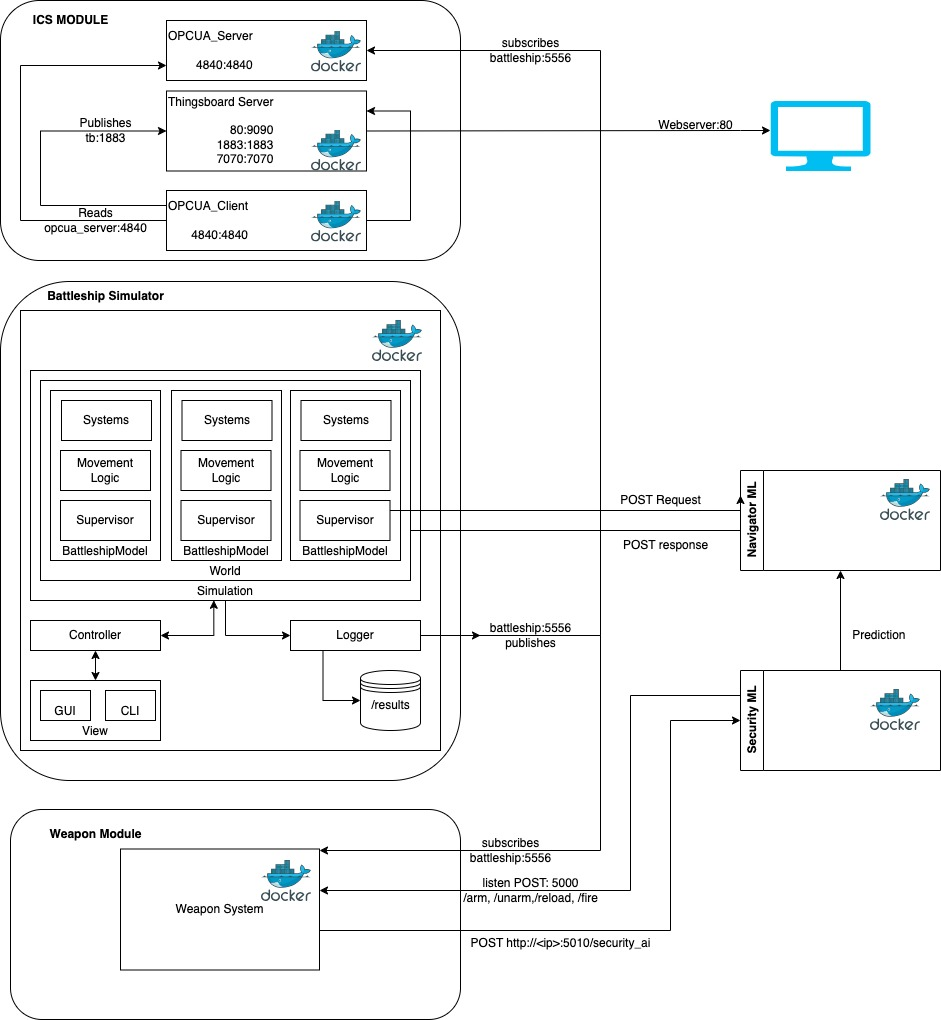
\includegraphics[width=0.84\linewidth]{communication_diagram_v2.png}
    \caption{Battleship Simulation Framework}
    \label{comms_diagram}
\end{figure} 
The experimental framework uses \textit{Python 3.9+} and third-party libraries to provide modeling, analysis, and simulation capabilities. The communications architecture described in \(Fig.~\ref{comms_diagram}\) facilitates modularity by employing microservice-based architecture for various functions such as scenario orchestration, environment representation, vehicle control logic, communications, data logging/transmission, and command line/graphical user interaction, where these components were containerized using \textit{Docker}-technologies. The Open Platform Communications Unified Architecture (OPC UA) and Message Queuing Telemetry Transport (MQTT) Framework also facilitated communication in industrial controls. The machine learning module incorporates many algorithms, such as decision trees, random forests, and reinforcement learning, utilizing the \textit{Scikit-Learn} and \textit{Flask} libraries. This modular simulation, system security, and AI integration facilitate the research of ensured autonomous marine vehicle operations.

\subsection{Battleship Operation}

BattleshipSimulator, an open-source library, models and predicts battleship threats using machine learning. Fossen \cite{b4} introduced physics-based movement modeling based on ship motion control concepts in \cite{b3}. Fig.~\ref{battleship_sim} shows the simulator autopilot navigating pathways and avoiding collisions.

\begin{figure}
    \centering
    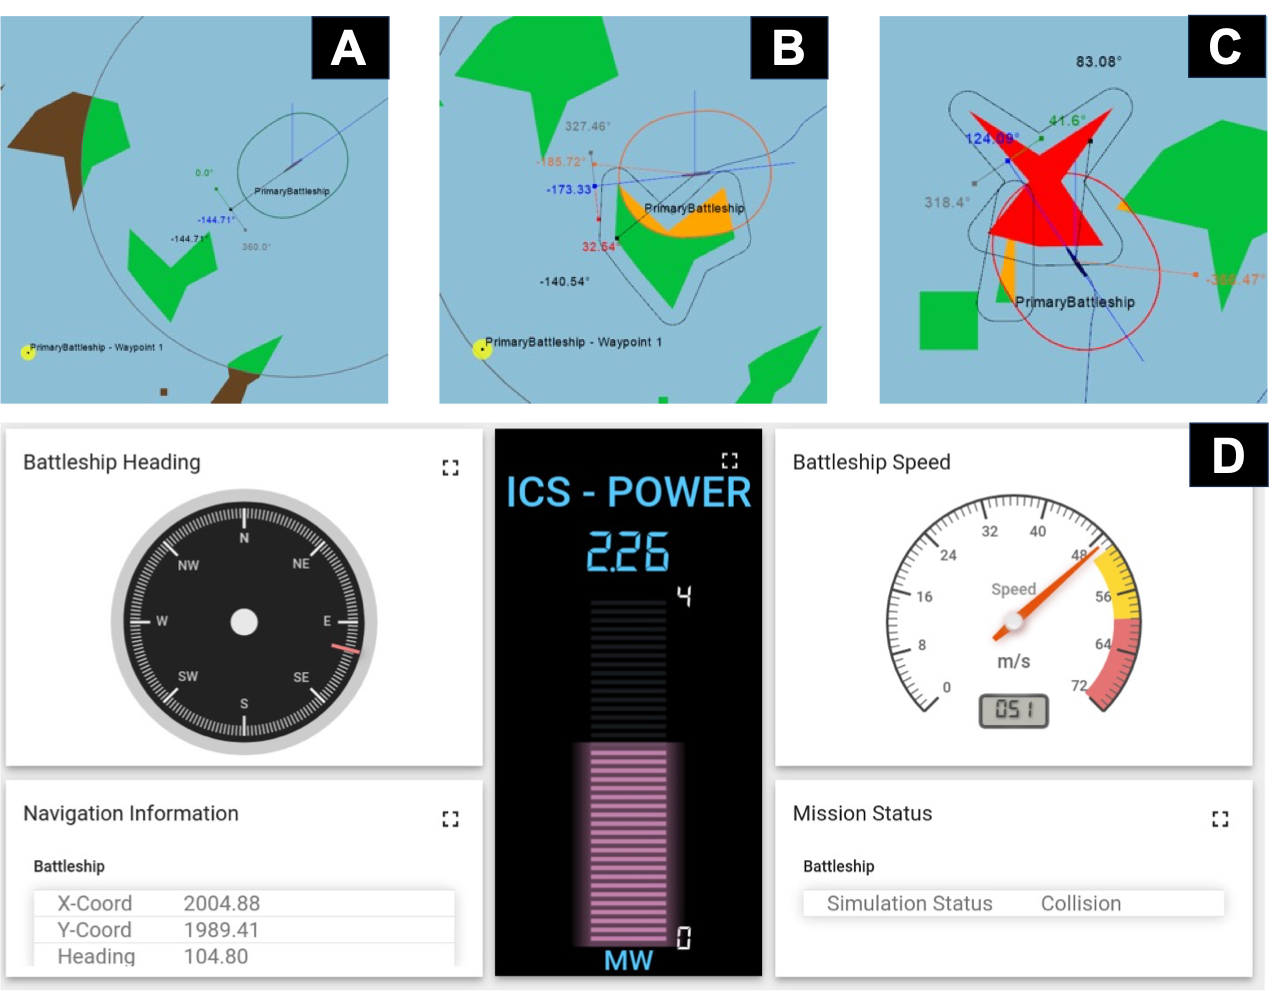
\includegraphics[width=1\linewidth]{dashboard_v2.png}
    \caption{BSS Collision State Reporting. (A) The battleship observes obstacles in its radar range (green), but none are close enough to pose an immediate threat. (B) As the battleship moves towards Waypoint \#1, obstacles come within a pre-defined "minimum safe area" and may pose an immediate threat. (C) The battleship collides with an obstacle (red), it can no longer move, and the scenario is considered a failure. (D) The \textit{OPC UA} Server Dashboard collects information regarding Speed, Power, Coordinates, and AI Status.}
    \label{battleship_sim}
\end{figure}


BSS has collision avoidance, a simple heuristic to turn away from objects, and waypoint tracking battleship navigation that can be overridden. Testing settings use procedural terrain generation with random waypoints and obstacles. BSS's modular ICS network decoupling allows independent physics modeling, a significant benefit for this research. High-fidelity battleship modeling and modular architecture enable extensible autonomous marine vehicle security evaluation.

\subsection{ICS Network}
To reproduce attacks on the BSS and improve data authenticity, an ICS network is required Fig.~\ref{battleship_sim}. An \textit{OPC UA} uses ICS data. In network-constrained situations, \textit{MQTT} offers efficient and lightweight communications. Using `opcua` for \textit{OPC UA} server and `paho.mqtt` for \textit{MQTT} client, the module seamlessly integrates with BSS. Data is instantaneously exchanged and synchronized between the logger function and \textit{ZeroMQ} server, guaranteeing simulator integrity and responsiveness. Dual technology integrates modules into the BSS system, allowing internal and external communication. The modular design is tested with a power generation module in the ICS network.

BSS uses the simple ICS power generator module to mimic power production. This module calculates the battleship power based on the ship's speed, drag, and navigation data.   The power-generating computational formula carefully considers drag coefficient, water density, cross-sectional area, and battleship velocity. The power calculation in the ICS module utilizes fluid mechanics coefficients to model naval power dynamics. The model applies a seawater density of 1025 $kg/m^3$, a drag coefficient of 0.035, and a cross-sectional area of 1005 $m^2$ \cite{b14}.

A \textit{Python} script calculates the simulated power required for the battleship's movement by first computing the drag force acting on the vessel \eqref{drag_eq}. This is achieved using the formula:
\begin{equation}
force_{drag} = 0.5 (c_d )(\rho) (area) (speed) 
\label{drag_eq}
\end{equation}
where \( c_d \) represents the drag coefficient, \( \rho \) is the density of seawater, \( \text{area}_{m^2} \) is the cross-sectional area facing the fluid flow, and speed (m/s) is the ship's speed in meters per second. Subsequently, the power is determined by multiplying this drag force by the ship's speed, providing the power in watts needed to 
overcome the drag and maintain the current speed. 
This module replicates power output changes and creates a realistic environment for analyzing and forecasting the SM-ML features. The SM-ML needs this module to detect cybersecurity and operational issues that can affect power emissions in a battleship. 

\subsection{Weapon System}
The weapons simulator emulates a system that takes manual commands and decides actions based on certain environment variables. Just as a Close-In Weapon System (CIWS) used to defend against anti-ship missiles and other close threats, the emulated weapon system can decide when to fire based on the real-time distance between the battleship and the target, based on the coordinates provided by the navigation system.  

The simulation considers weapon range to simulate real-life systems and arm/disarm/fire based on the change in value of the range. The distance to the target is calculated by a \textit{Python} script that considers the battleship and targets current \texttt{x} and \texttt{y} coordinates using the formula \eqref{wpn_distance}, and Fig.~\ref{WPNlogic} depicts the logic on actions to take based on the distance to the target.

\begin{equation}
\text{distance} = \sqrt{(x_2 - x_1)^2 + (y_2 - y_1)^2}  
\label{wpn_distance}
\end{equation}

The simulation allows user input using the ingress POST Application Programming Interface (API) and uses egress POST requests to update the SM-ML with all the tasks and decisions. This makes it crucial to verify if there is any cybersecurity-related abnormality and, based on observation, take decisions to change the course of action. This modularity increases the simplicity of simulating cyber attacks against the weapons system according to a STRIDE threat model.

\begin{figure}
    \centerline{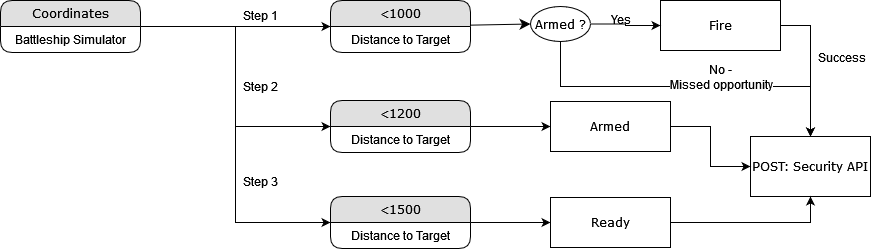
\includegraphics[width=1\linewidth]{firinglogic.png}}
    \caption{Weapon System Automated Firing Logic}
    \label{WPNlogic}
    
\end{figure}

% -----------------------------------------------------------------------
\section{Threat Model}
Advancements in AI have led to an increasing number of autonomous systems and controls put into place in many areas. This paper focuses on autonomous naval vehicles and how these autonomous systems are vulnerable to cyber-attacks. This problem is well researched with several threat models and cyber intrusions being performed as in \cite{b8}. 

\subsection{Attack Background}
According to the IACS recommendation on cyber resilience \cite{b13}, functional failures related to the control system's operation, propulsion, and steering can cause high integrity and availability risks. Thus providing the reason that the cybersecurity of a ship must be considered. There are many attacks against the cyber systems of naval vessels, but to consider a few: GPS attacks, firmware hacks, Denial of Service (DOS) attacks, Automatic Identification System (AIS) attacks, Electronic Chart Display and Information System (ECDIS) attacks \cite{b1}. While there are a myriad of other attacks, the focus of this paper will be on GPS and firmware-based attacks. These attacks have proven possible and can be easy to exploit. GPS signals come from orbiting satellites, are weak enough for attackers to interfere, and can be easily overpowered. GPS spoofing will impact navigation and cause sequence problems, such as late or missed shots of the weapon system. Firmware-based attacks are typically performed using malicious programs that manipulate hardware in an unauthorized manner. The key examples related to this paper are power control ICS and weapon targeting systems, which could be spoofed or manipulated with malware. 

\subsection{STRIDE Threat Model: Current and Potential Attacks}
A risk assessment was performed based on STRIDE Threat Modeling principles to demonstrate the modular capabilities implemented in this paper, similar to \cite{b8}. This assessment describes some current and potential attacks the simulator can model. The STRIDE Threat Model is described in Table \ref{tab:STRIDE} and is used to describe a variety of potential attacks using a threat.

The actual attacks used in this paper were to spoof the GPS data for the vessel; this was simulated by changing the location of the BSS. For the weapon targeting system, a tampering attack was simulated by altering the parameters of the weapon system. Finally, for the power control ICS, another tampering attack was simulated by altering power ICS data.


\begin{table}
\centering
\caption{STRIDE Threat Model}
\label{tab:STRIDE}
\scriptsize 
\setlength{\tabcolsep}{2pt} 
\begin{tabular}{
  |>{\centering\arraybackslash}m{1.5cm}
  |>{\centering\arraybackslash}m{1.5cm}
  |>{\centering\arraybackslash}m{4cm}|}
\hline
Threat Category      & Security Tenet Violated & Definition                                                \\ \hline
Spoofing               & Authenticity    & An adversary capability to mask as another entity or pass data as authentic \\ \hline
Tampering            & Integrity               & An adversaries capability to alter data inside the system \\ \hline
Repudiation          & Non-repudiation         & The inability to attribute actions with evidence          \\ \hline
Information Disclosure & Confidentiality & Revealing information to those without proper permissions                     \\ \hline
Denial of Service      & Availability    & Taking down the system and removing the availability/operation of the system  \\ \hline
Privilege Escalation & Authority               & Executing unauthorized protocols or programs              \\ \hline
\end{tabular}%
\end{table}


% ----------AI Navigation Monitor-------------------------------------
\begin{table}
\centering
\caption{Feature Descriptions for Battleship Simulation}
\label{tab:feature_descriptions}
\begin{tabular}{@{}p{8cm}@{}}
\toprule
\textbf{Description of Selected Features} \\
\midrule
\textbf{desired\_heading:} Direction battleship is trying to move towards  \\
\textbf{option\_port:} Status option for the port side of battleship  \\
\textbf{out\_of\_bounds:} Indicates ship movement outside simulation boundary  \\
\textbf{RadarSonar.collision\_warning:} Warning for potential collisions  \\
\textbf{RadarSonar.collision\_event:} Indicates collision occurrence  \\
\textbf{Engine.desired\_speed:} Desired speed of the battleship  \\
\textbf{Distance\_to\_point\_1:} Distance to waypoint 1  \\
\textbf{Distance\_to\_point\_2:} Distance to waypoint 2 \\
\textbf{Distance\_to\_point\_3:} Distance to waypoint 3  \\
\textbf{Distance\_to\_point\_4:} Distance to waypoint 4 \\
\textbf{Distance\_to\_radar\_obj\_1:} Distance to object 1 detected by radar  \\
\textbf{Distance\_to\_radar\_obj\_2:} Distance to object 2 detected by radar \\
\textbf{Distance\_to\_radar\_obj\_3:} Distance to object 3 detected by radar  \\
\textbf{Distance\_to\_radar\_obj\_4:} Distance to object 4 detected by radar  \\
\textbf{Direction\_port:} Direction for next move (port)  \\
\textbf{Direction\_starboard:} Direction for next move (starboard)  \\
\textbf{Security\_ML:} Security status from SM-ML  \\
\bottomrule
\end{tabular}
\begin{minipage}{0.44\textwidth}
\footnotesize This table summarizes the key features used to train the AI-NM.
\end{minipage}
\end{table}

\section{AI Navigation Monitor}
The AI-NM utilizes the Navigator-ML and BSS information to make battleship decisions. Navigator-ML is trained to predict battleship heading and speed similar to BSS native navigation and is used by AI-NM to check BSS behavior continuously.
\subsection{Features and Modeling}
Navigator-ML is trained on BSS native navigation and SM-ML outputs to predict battleship heading and speed. The datasets from BSS are preprocessed by removing missing values and dropping columns with high correlation based on the heatmap we developed. Columns with categorical and boolean values are converted using one-hot encoding. Additionally, features are extracted by calculating Euclidean distance between current battleship coordinates and waypoints. Final features are listed in Table \ref{tab:feature_descriptions}.

The dataset is divided into 80\% for training and the remaining 20\% for testing. The model is trained using three algorithms: Decision Tree, Random Forest, and KNN Regression. All three models' hyperparameters are tuned using Grid-Search CV and a cross-validation set of 5. 

\subsection{Training}
Mean Absolute Error (MAE) is the total of absolute differences between expected and actual values divided by observations. MAE outputs y-units. The regression loss function uses Mean Square Error (MSE), the most common regression metric, to calculate the squared error between predicted and actual values. R2 is the only context-independent model comparison metric. 
Regression models Decision Tree, Random Forest, and K-Nearest Neighbors predicted Battleship navigation. Performance measurements were MAE, MSE, and R-squared. The Decision Tree model was more accurate and precise, with an MAE of 0.1688 and an MSE of 0.3578. With 0.9999 R-squared, it accounts for variance well. The Random Forest model lost effectiveness as errors rose. MAE and R-squared for KNN matched Decision Tree. But MSE was greater. Decision Tree model performed better in navigation challenge accuracy and dependability, indicating its applicability. The Decision Tree was best for this scenario because of its lesser computational effort and faster forecasts without normalizing or scaling. 



% ---------Security Navigation Monitor------------------------------------
\section{Security Navigation Monitor}
The SM-ML Module uses real-time data from components to monitor their behaviors and functionality. The SM-ML was inspired by using Explainable AI to filter anomalous system component behavior and take action against it by classifying those behaviors by quantifying their system impact and defining their reasoning using these metrics. This approach aims to be preventive, explainable \cite{b5}, robust in spotting new threats and anomalies, and less dependent on humans. 
Data Collection and Preparation: The data is integrated from the ICS Module and the Weapon System. The information these systems provide is crucial for the SM-ML since it contains the parameters critical to the battleship's operational stability. 


\subsection{Features and Modeling}
The suggested cybersecurity architecture employs the 'DecisionTreeClassifier' model for training, as it can distinguish between three system functionality states. All systems operate optimally in State ``1'', or ``Go''. State ``2'' or ``Down'' implies the weapon system is non-operational, but the ICS module works. State ``3'' indicates a compromise that may affect the ICS module, weapon system, or both. These states act as a ``Label'' column classified as operational (1), compromised (3), or non-operational (2). Data was generated from compromised and non-compromised ICS modules and weapon systems for training purposes and labeled accordingly.
The Final features are described in Table \ref{tab:sec_feature}. 
\begin{table}
\centering
\caption{Features for Security Navigator ML}
\label{tab:sec_feature}
\begin{tabular}{cl}
\toprule
\textbf{S. No.} & \textbf{Selected Features Name} \\
\midrule
1 & Power Required (Watts, obtained from ICS Module \\
2 & Weapon Range Status \\
3 & Weapons Status  \\
4 & Msg (Encoded message from Weapon System) \\
\bottomrule
\end{tabular}
\begin{minipage}{0.44\textwidth} 
\footnotesize Key features selected during the training of the SM-ML system.
\end{minipage}
\end{table}

Transparency and speed are essential for understanding the model's decision-making process in a trustworthy domain in the context of real-time security, which the decision tree graph provides effectively by handling non-linear relationships and complex feature interactions while being quick to train.

\subsection{Training}
Three machine-learning classification models were used to assess the SM-ML system: Decision Tree, Random Forest, and KNN. Each model was thoroughly examined to discover the best fit for our purpose. 

Three machine learning models—Decision Tree, Random Forest, and K-Nearest Neighbors—are compared in this article. The efficacy of the models was assessed using various metrics, including precision, recall, F1 score, and accuracy. Regarding overall performance, the Decision Tree model demonstrated superior precision, recall, and F1 scores of 1.0 and accuracy of 0.998. This suggests that the threat detection and classification capabilities are exact. The Random Forest model performed admirably, albeit marginally inferior. The performance of the KNN model was considerably inferior across all metrics. The findings indicate that the Decision Tree model exhibited superior performance compared to the other two models, showcasing the highest levels of accuracy and dependability in anomaly detection. It validates quantitatively the Decision Tree's efficacy as a security monitoring model.

% -----------------------------------------------------------------------
\section{Experimental Evaluation}
\subsection{Experimental Setup}

The simulator and the AI models were developed on a Windows-based Operating System with an 11th Gen Intel Core i5 processor and 16GB RAM and used \textit{Python 3.9+}. It uses microservices and third-party libraries for scenario generation, environment modeling, data transmission, and user interaction. \textit{Arcade, Shapely, PyYAML, Numpy, ZeroMQ, OPC UA, MQTT, Scikit-Learn}, and \textit{Flask} were used. The modular, containerized design allows simulation, analysis, and data flow orchestration with \textit{Docker}-based technologies. 


\subsection{Experimental Procedure}
Three primary sets of experiments were run in our study. First, we tested the native navigator's ability to avoid collisions. Next, we tested the ability of the AI navigation monitor to take over and either avoid collisions on behalf of the native navigator or stop the ship before a collision. Finally, we test the AI security monitor's ability to identify anomalies in the ICS network.
\subsubsection{Native Navigator}
To test the effectiveness of the BSS native navigation, a set of 10 scenarios was pseudo-randomly generated. These scenarios were then run with and without the native navigation to provide a suitable comparison. The results of these ten scenarios were tabulated and displayed in the first column in Table \ref{tab:battleship_scenario}. 
\subsubsection{AI Navigation Monitor}
The AI-NM utilizes the Navigator-ML and BSS information to make battleship decisions. The following logic is implemented for AI-NM in a series of steps. The first step is the AI-NM continuously compares the BSS heading to Navigator-ML predictions. It triggers alerts and halts the ship if the BSS starts heading in a strayed-off direction. In the second step, AI-NM initiates the Collision Avoidance Supervisor when Collision Avoidance warnings are validated, and Navigator-ML predicts values consistent with the BSS. In the final step, AI-NM brings the battleship to speed zero when Navigator-ML forecasts zero speed, signaling a potential security compromise by SM-ML. The results of these 10 scenarios were tabulated and displayed in Table \ref{tab:battleship_scenario}, the second column.
\subsubsection{Security Monitor ML}
We ran the trained 'DecisionTreeClassifier' model against data from a compromised weapon system and ICS module to determine its ability to identify anomalous behavior. The accuracy of SM-ML's prediction is described in the Table \ref{tab:sec_expeval}.

% -----------------------------------------------------------------------
\section{Results and Discussion}
 In this work, we demonstrate how our battleship simulator can simulate multiple algorithms and techniques to avoid collisions and how other components of the battleship, like the ICS and weapon system, communicate and work in harmony. Monitoring the battleship simulator is two ML-based systems that automatically control different components when needed. The section below describes the results generated by each element individually. 
\begin{table}
\centering
\caption{Battleship Scenario Analysis}
\label{tab:battleship_scenario}
\footnotesize % This command will make the text size of the table smaller
\begin{tabular}{@{}c>{\centering\arraybackslash}p{1.6cm}>{\centering\arraybackslash}p{1.6cm}>{\centering\arraybackslash}p{1.6cm}>{\centering\arraybackslash}p{1.6cm}@{}}
\toprule
\# & Native Navigator & Navigation AI & Navigation AI Attacked \\ \midrule
1  & Collision & Avoided &Halted\\
2  & Collision & Avoided &Halted\\
3  & Collision & Collision &Halted\\
4  & Collision & Avoided &Halted\\
5  & Collision & Avoided &Halted\\
6  & Collision & Avoided &Halted\\
7  & Collision & Avoided &Halted\\
8  & Collision & Avoided &Halted\\
9  & Collision & Collision &Halted\\
10  & Success & Success &Halted\\
\bottomrule
\end{tabular}
\begin{minipage}{0.48\textwidth} % You can change the width (0.8\textwidth) as needed
\footnotesize The results of simulated attack on a battleship. 'Fail' indicates a scenario where the ship collided with an obstacle, while 'Success' denotes successful navigation. 'Avoided' indicates the AI-NM and the collision avoidance prevented a collision. 'Halted' indicates that the AI-NM stopped the ship once the  SM-ML sent a compromise signal.
\end{minipage}
\end{table}
\subsection{Results of Native Navigation in BSS}
As shown in Table \ref{tab:battleship_scenario}, the native navigation on the battleship does not show significant success rate for each scenario. This native navigation allows some object avoidance, which is expected considering the simple steering heuristic. 

\subsection{AI Navigator Monitor}
The AI-NM stopped the battleship when Navigator-ML gave a speed zero response as per SM-ML's prediction of a compromise. Additionally, AI-NM alerted the system when BSS gave anomalous headings compared to Navigator-ML.

The trained Decision Tree Model is serialized and stored in binary format. The model predicts the heading based on data from the BSS and the Security ML model. The Navigation AI pre-processes the records, predicts heading and current speed values, and returns the information to the BSS. For example, suppose the ship's heading deviates from the native navigator (over a 2-degree difference). In that case, the AI will predict the heading and perform a logic comparison to initiate the collision avoidance algorithm if needed.  Otherwise, the Navigation AI will send a stop signal.

Table \ref{tab:battleship_scenario} shows that the Navigation AI avoided collisions and successfully navigated in 7 of 9 cases (77.7\%). This demonstrates the improved navigation capabilities of the AI system compared to the basic native controls. However, in scenarios 3 and 9, even the Navigation AI resulted in collisions, perhaps due to limitations in sensing obstacles or control responses.

Scenario 10 shows the Native Navigator and Navigation AI succeeding, implying a less complex navigation task.  The crucial role of the AI Navigator Monitor here is to monitor for anomalies and compromise signs to intervene during failures. Every time the AI-NM receives a compromise signal from the SM-ML, it halts the BSS. By predicting compromises and controlling navigation this way, the AI Navigator Monitor acts as an oversight system to catch navigation AI failures and prevents accidents even when collisions cannot be entirely avoided.


\subsection{Security Navigator Monitor}
The Security AI successfully predicted over 1000 cases of potential compromises when it received anomalous power values from a simulated cyber attack on the ICS Network Module. The simulator read falsely because sensor systems received fake environmental data in this attack scenario. Every Weapon System task generated status data that indicated inconsistencies when failures or faults occurred. A manual “fire” command may miss the target out of range, or a missile firing request may fail if it is unloaded. In the scenario, the Security AI received manipulated targeting data to lock onto erroneous targets, imitating an attack.
Table \ref{tab:sec_expeval} displays the Security AI's capacity to anticipate Weapon System breach situations. When anomalous ICS network power values suggested a cyber assault, 1000 predictions were successful. Other circumstances like missile misses and out-of-range status were mostly anticipated correctly. The only exception was the “Missile Not Loaded” case, which saw 38 failed predictions out of 252 cases, representing an approximately 15\% failed prediction rate. The overall accuracy of Security AI prediction stood at approximately 98.5\%.


\begin{table}
\centering
\caption{Experiment Result of Compromised Weapon System}
\label{tab:sec_expeval}
\footnotesize % This command will make the text size of the table smaller
\begin{tabular}{@{}c>{\centering\arraybackslash}p{2.8cm}>{\centering\arraybackslash}p{1.2cm}>{\centering\arraybackslash}p{1.2cm}>{\centering\arraybackslash}p{1.2cm}@{}}
\toprule
\textbf{S. No.} & \textbf{Case of Compromise} & \textbf{Success} & \textbf{Failure} & \textbf{Total} \\ 
\midrule
1 & No More Rounds & 500 & 0 & 500 \\
2 & Out of Range & 392 & 0 & 392 \\
3 & Miss & 134 & 0 & 134 \\
4 & Loading & 214 & 38 & 252 \\
5 & Reloading & 215 & 0 & 215 \\
6 & Power & 1000 & 0 & 1000 \\
\bottomrule
\end{tabular}
\begin{minipage}{\columnwidth}
\footnotesize Outcomes of various compromise scenarios in a weapon system such as missile misses, sudden out-of-range status, empty rounds status, or unusual ICS system power due to compromise. 
\end{minipage}
\end{table}

 



% -----------------------------------------------------------------------
\section{Limitations}
BSS modules are still a work in progress with the potential to simulate threats against semi-autonomous or fully autonomous naval vehicles. The modules' capabilities are expandable and modular but currently limited. The BSS can simulate additional ships according to \cite{b4}. However, this research is limited to a specific class and type. The native collision avoidance algorithm is easy to replace but a simple heuristic prone to failure. This collision avoidance is also a limiting factor for the AI-NM since the ML is trained on a simple collision avoidance algorithm. The SM-ML is limited by the relatively small amount of systems stored in the ICS network simulation.


% -----------------------------------------------------------------------
\section{Summary and Future Work}
This investigative study demonstrates the feasibility of developing a modular battleship simulator and an associated AI navigation and security monitoring system. Even though our work had limitations, we have shown that such a feat is feasible. This work is a contribution to the literature on maritime vehicle simulators and also maritime systems cybersecurity.

Future work could expand the simulation modules and threat model to focus on real-world problems in autonomous maritime platforms and control systems. 

%-----------------TABLES AND FIGURES--------------------------------

\begin{thebibliography}{00}
\bibitem{b1} J. M. Lanouette, ``Naval Cyber Warfare -- Are Cyber Operators Needed on Warships to Defend against Platform Cyber Attacks,’’ Master's thesis, Canadian Forces College, Toronto, Ont., Canada, 2016, JCSP/PCEMI 42-17.

\bibitem{b2} J. Coker. (2023), "1000 Shipping Vessels Impacted by Ransomware Attack," in Infosecurity Magazine, 18 January 2023. Available: \url{www.infosecurity-magazine.com/news/shipping-vessels-ransomware-attack}

\bibitem{b3} T. I. Fossen (2021). Handbook of Marine Craft Hydrodynamics and Motion Control. 2nd. Edition, Wiley.

\bibitem{b4} T.I. Fossen (2023) Python Vehicle Simulator Software. Available: \url{github.com/cybergalactic/PythonVehicleSimulator/tree/master}

\bibitem{b5} V. Manoj et al, (2023) "Explainable autonomic cybersecurity for industrial control systems," in 2023 IEEE 13th Annual Computing and Communication Workshop and Conference (CCWC).

\bibitem{b6} T. C. My, L. D. Khanh, and P. M. Thao,``An Artificial Neural Networks (ANN) Approach for 3 Degrees of Freedom Motion Controlling,’’ in International Journal on Informatics Visualization, vol. 7, no. 2, pp. 301-309, Jun. 2023.

\bibitem{b7} Y. Suo, S. Yang, G. Chen, and W. Liu, "A Target Ship Server Driven by AIS Signal for the Navigation Simulator," in ``2017 2nd International Conference on Computational Modeling’’, Simulation and Applied Mathematics (CMSAM 2017), Xiamen, Fujian, China, 2017, pp. 76-82, ISBN: 978-1-60595-499-8.

\bibitem{b8} Kavallieratos, G., Katsikas, S., Gkioulos, V. (2019). Cyber-Attacks Against the Autonomous Ship. In: Katsikas, S., et al. Computer Security. SECPRE CyberICPS 2018. Lecture Notes in Computer Science(), vol 11387. Springer, Cham.

\bibitem{b9} K. Hasegawa, J. Fukuto, R. Miyake, and M. Yamazaki,``An Intelligent Ship Handling Simulator with Automatic Collision Avoidance Function of Target Ships,’’ in Proceedings of the 17th International Navigation Simulator Lecturers’ Conference (INSLC 17), Rostock-Warnemuende, Germany, 2012.

\bibitem{b10} Raphael Zaccone and Michele Martelli (2020) A collision avoidance algorithm for ship guidance applications, Journal of Marine Engineering and Technology, 19:sup1, 62-75. 

\bibitem{b11} J. M. Szatkowski, Y. Li, and L. Du, "Enabling Reconfigurable Naval SCADA Network through Software-Defined Networking," 2022 IEEE Transportation Electrification Conference and Electric Aircraft Technologies Symposium (ITEC+EATS), 2022, pp. 214-218.

\bibitem{b12} L. Watkins, D. Hamilton, K. Kornegay, and A. Rubin. (2021). ``Triaging Autonomous Drone Faults By Simultaneously Assuring Autonomy and Security,'' in 2021 55th Annual Conference on Information Sciences and Systems (CISS), 2021, pp. 1-6, doi: 10.1109/CISS50987.2021.9400286.

\bibitem{b13} IACS (2022). Rec 166 – Recommendation on Cyber Resilience – New Corr.2 Apr 2022 Clean. Available: \url{https://iacs.org.uk/resolutions/recommendations/161-180/rec-166-new-corr2-cln}

\bibitem{b14} D. S. Cusanelli and G. Karafiath, (2012) "Hydrodynamic Energy Saving Enhancements for DDG 51 Class Ships," in ASNE Day 2012, 2012, pp. 1-16.
\end{thebibliography}
\vspace{12pt}

\end{document}
